

\subsubsection{フロアマップを用いた初期進行方向の補正}

% TODO 段落が短すぎる
図\ref{fig:pdr-remove-drift}では,軌跡の初期進行方向の誤差の問題がある.初期進行方向の誤りは,その後の全ての推定位置に影響を与え,実際の移動経路から大きく逸脱する原因となる.この問題を解決するため,マップマッチングによる初期方向補正機能を実装しており,MapMatchCorrectorクラスとして提供している.

MapMatchCorrectorクラスの利用例をListing\ref{lst:rotate-trajectory-using-floormap}に示す.
このクラスに必要な情報はフロアマップ情報である.フロアマップは
建物の構造を表す2次元の画像データとして与えられ,歩行可能な領域と
歩行不可能な領域を区別できる必要がある.図\ref{fig:floor-map}に実際の
フロアマップを示す.このマップでは灰色の部分が歩行可能領域,白色の部分が
歩行不可能領域を表している.
% TODO: 文章がちらばっている意味がわからない:要修正
このクラスは,フロアマップの構造的特徴を利用して最適な初期進行方向を
推定する.この手法は,多くの屋内環境において壁や通路が直交する特徴を活用する.
図\ref{fig:floor-map}に示した実際のフロアマップでは,
歩行可能な経路の多くが建物の主軸に沿って配置されている.

% TODO: 2.修正関数の呼出しの部分は削除したがそれでよかったのだろうか
% TODO: 2.captionの名前は検討した方がいいかも
\begin{lstlisting}[caption={MapMatchCorrectorの使用例},label=lst:rotate-trajectory-using-floormap,float=ht]
# フロアマップの読み込み
floor_map = FloorMap(
    floor_name="floor_5",
    floor_map_path="floor_5.png",  # 二値化された画像
    dx=0.01,  # x方向の1ピクセルあたりの距離(m)
    dy=0.01   # y方向の1ピクセルあたりの距離(m)
)

# MapMatchCorrector の初期化
map_match_corrector = MapMatchCorrector(
    pdr_estimator=estimator,
    floor_map=floor_map
)
\end{lstlisting}


\begin{figure}[H]
	\centering
	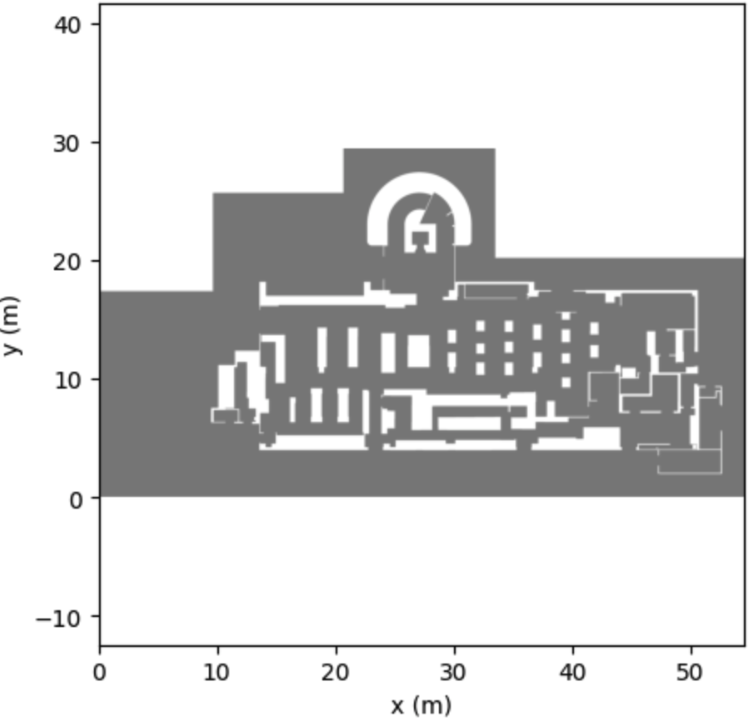
\includegraphics[width=\linewidth]{../image/floor-map.jpg}
  \caption{フロアマップ情報} \label{fig:floor-map}
\end{figure}

初期進行方向の推定は,二段階のプロセスで行われる.
第一段階では,軌跡のx軸,y軸に対して平行な成分の割合を最大化する角度を探索する.
具体的には,進行方向の角度が垂直方向(90度または270度)に対して±0.1ラジアン以内,
または水平方向(0度または180度)に対して±0.1ラジアン以内の歩行ステップを平行な
成分としてカウントする.
この閾値は,人間の通常の歩行では廊下や通路に対して完全に平行でなくとも,
おおむねその方向に沿って歩く傾向を考慮して設定されている.
図\ref{fig:parallel}は,異なる回転角度での軌跡における平行成分の分布を比較したものである.
赤い点はx軸またはy軸に対して平行な成分を,青い点はそれ以外の成分を示している.
左側の例では平行な成分の割合が少なく,軌跡が建物の主軸に対して斜めに配置されている.
一方,右側の例では平行な成分の割合が多く,軌跡が建物の構造とよく整合している.
このように,平行成分の割合を分析,建物の主軸に整合する可能性の高い
角度を特定できる.ただし,この情報だけでは4つの候補角度(0度,90度,180度,
270度)のうち,どの角度が最適であるかを一意に決定できない.
% NOTE ここよく考える最初から90,180,240,270度なの決まってないかな?.
% じゃあ最初から90,180,240,270度に回転させたらって思ったけど,どこを回転の基準にするのかわからないから無理そう?

\begin{figure}[H]
	\centering
	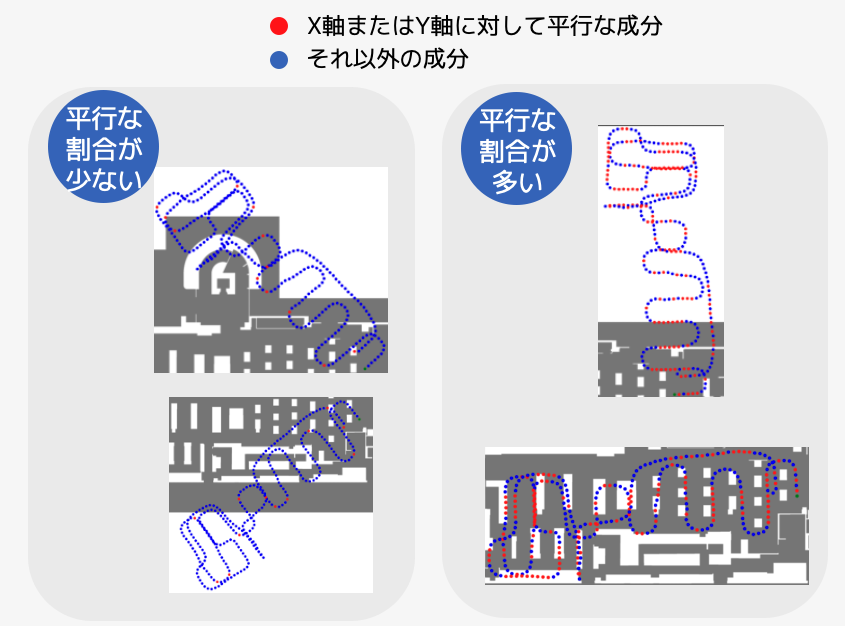
\includegraphics[width=\linewidth]{../image/parallel.jpg}
	\caption{x軸とy軸に対して平行な成分の割合}    \label{fig:parallel}
\end{figure}


第二段階では,フロアマップ上の歩行可能領域の情報を用いて最適な角度を決定する.
具体的には,第一段階で特定した各候補角度ごとに軌跡を回転させ,その軌跡上の点がフロアマップ上の歩行可能領域に含まれる割合を計算する.
この計算により,もっとも建物構造と整合する角度の特定が可能となる.
図\ref{fig:pdr-rotate}は,この2段階の補正処理を適用した結果を示しており,補正後の軌跡は建物の構造に整合し,正解軌跡により近い形状となっている.
この手法は特に廊下や部屋が格子状に配置された一般的なオフィスビルなどの環境で効果的に機能する.ただし,円形建築物やオープンスペースが多い環境では,建物の主軸が明確でないため,補正効果が限定的となる可能性がある.


\begin{figure}[H]
	\centering
	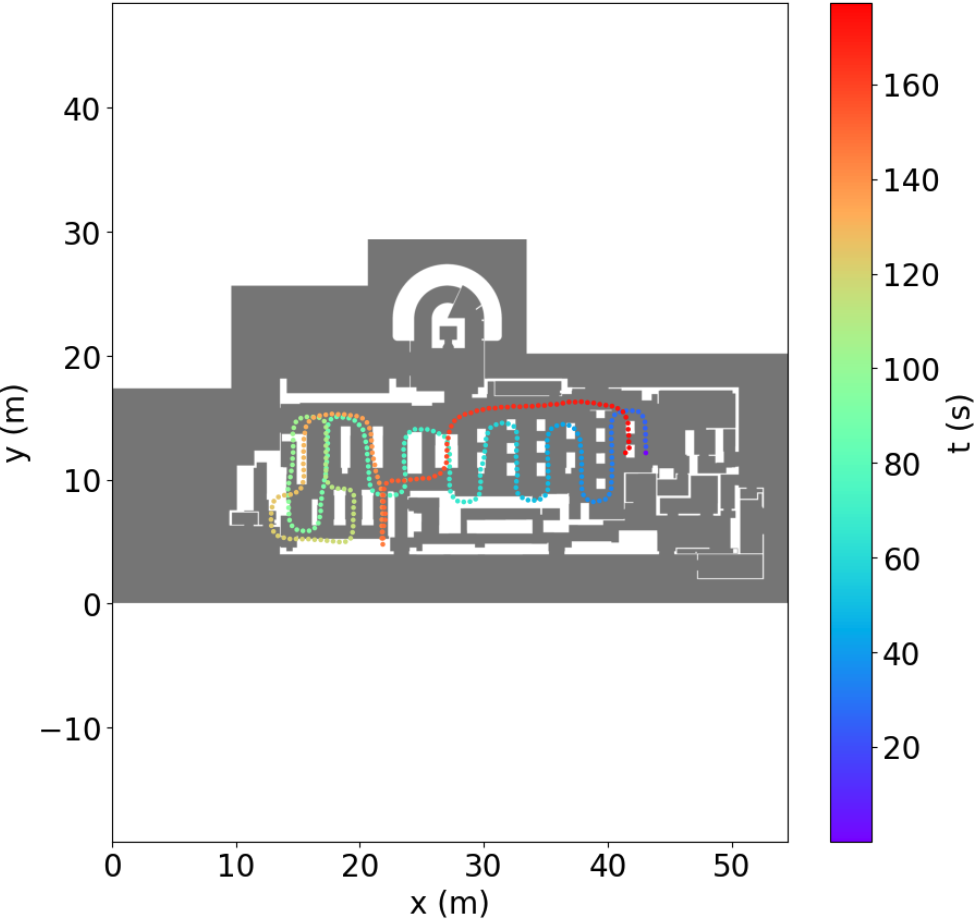
\includegraphics[width=\linewidth]{../image/pdr-rotate.jpg}
	\caption{初期進行方向の補正後の軌跡}    \label{fig:pdr-rotate}
\end{figure}



